%  article.tex (Version 3.3, released 19 January 2008)
%  Article to demonstrate format for SPIE Proceedings
%  Special instructions are included in this file after the
%  symbol %>>>>
%  Numerous commands are commented out, but included to show how
%  to effect various options, e.g., to print page numbers, etc.
%  This LaTeX source file is composed for LaTeX2e.

%  The following commands have been added in the SPIE class 
%  file (spie.cls) and will not be understood in other classes:
%  \supit{}, \authorinfo{}, \skiplinehalf, \keywords{}
%  The bibliography style file is called spiebib.bst, 
%  which replaces the standard style unstr.bst.  

\documentclass[draft]{spie}  %>>> use for US letter paper
%%\documentclass[a4paper]{spie}  %>>> use this instead for A4 paper
%%\documentclass[nocompress]{spie}  %>>> to avoid compression of citations
%% \addtolength{\voffset}{9mm}   %>>> moves text field down
%% \renewcommand{\baselinestretch}{1.65}   %>>> 1.65 for double spacing, 1.25 for 1.5 spacing 
%  The following command loads a graphics package to include images 
%  in the document. It may be necessary to specify a DVI driver option,
%  e.g., [dvips], but that may be inappropriate for some LaTeX 
%  installations. 
\usepackage[]{graphicx}
\usepackage[percent]{overpic}
% \usepackage[authoryear]{natbib}

% \title{Validation of the MoB-ELM Atmospheric Correction Algorithm for Landsat 8 over Case 2 Waters} 

\title{Atmospheric Correction for Landsat 8 over Case 2 Waters}

%>>>> The author is responsible for formatting the 
%  author list and their institutions.  Use  \skiplinehalf 
%  to separate author list from addresses and between each address.
%  The correspondence between each author and his/her address
%  can be indicated with a superscript in italics, 
%  which is easily obtained with \supit{}.

\author{Javier A. Concha and John R. Schott
\skiplinehalf
Digital Imaging and Remote Sensig Lab\\Chester F. Carlson Center for Imaging Science\\Rochester Institute of Technology\\ 54 Lomb Memorial Dr., Rochester, NY 14623, USA\\
}

%>>>> Further information about the authors, other than their 
%  institution and addresses, should be included as a footnote, 
%  which is facilitated by the \authorinfo{} command.

\authorinfo{Further author information: (Send correspondence to Javier A. Concha)\\ E-mail: jxc4005@rit.edu, Telephone: 1-(585) 290-3145}%%>>>> when using amstex, you need to use @@ instead of @
 

%%%%%%%%%%%%%%%%%%%%%%%%%%%%%%%%%%%%%%%%%%%%%%%%%%%%%%%%%%%%% 
%>>>> uncomment following for page numbers
% \pagestyle{plain}    
%>>>> uncomment following to start page numbering at 301 
%\setcounter{page}{301} 

%% Added 07-29-15
\usepackage{multirow}% http://ctan.org/pkg/multirow
\usepackage{hhline}% http://ctan.org/pkg/hhline
\usepackage{epstopdf}
\epstopdfsetup{update} % only regenerate pdf files when eps file is newer
\usepackage{amsmath,epsfig}
\usepackage{hyperref}


\usepackage{tikz} % for flow charts
  \usetikzlibrary{shapes,arrows,positioning,shadows,calc}

\begin{filecontents*}{linereg.data}
#x y
0 4
10 24
\end{filecontents*} 

\begin{filecontents*}{linereg2.data}
#x y
2 8
8 20
\end{filecontents*}

\usepackage{url}

% Select what to do with todonotes: 
% \usepackage[disable]{todonotes} % notes not showed
\usepackage[draft]{todonotes}   % notes showed
\setlength{\marginparwidth}{2cm}
% \usepackage[textwidth=3.7cm]{todonotes}

% end of my packages
 
  \begin{document} 
  \maketitle 

%%%%%%%%%%%%%%%%%%%%%%%%%%%%%%%%%%%%%%%%%%%%%%%%%%%%%%%%%%%%% 
\begin{abstract}
Landsat 8 is a promising candidate to address the remote sensing of inland and coastal waters (Case 2 waters) due to its improved signal-to-noise ratio (SNR), spectral resolution, 12-bit quantization, and high spatial resolution. Atmospheric correction is essential for remote sensing of water since the signal from the water reaching the sensor is small compared to atmospheric scattering. Standard atmospheric correction algorithms fail over highly turbid Case 2 waters because the black pixel assumption, i.e. the signal leaving the water is zero beyond the near infrared (NIR), is not always satisfied. We developed a new atmospheric correction algorithm, the model-based ELM (MoB-ELM), for Landsat 8 imagery based on the empirical line method (ELM) that does not rely on the black pixel assumption. This algorithm uses pseudo-invariant features (PIF) from the image, ground-truth data, and water-leaving reflectances from an in-water radiative transfer model (Hidrolight) to determine reflectance and radiance values of the bright and dark pixels used in the ELM method.  We compare the results with in situ remote sensing reflectance measurements for different water bodies that exhibit a range of optical properties. We calculate reflectance errors for each band taking the in situ data as ground-truth, and then compare them to results from standard atmospheric correction algorithms. These reflectance errors are small in all the visible bands for a wide range of concentrations. These results show that our atmospheric correction algorithm allows one to use Landsat 8 to study Case 2 waters as an alternative to traditional ocean color satellites (e.g. MODIS, SeaWiFS). 
\end{abstract}

%>>>> Include a list of keywords after the abstract 
\keywords{Atmospheric Correction, Case 2 Water, Landsat 8, Inland and Coastal Water, Empirical Line Method, Operational Land Imager, OLI, Ocean Color}


%%%%%%%%%%%%%%%%%%%%%%%%%%%%%%%%%%%%%%%%%%%%%%%%%%%%%%%%%%%%%
\section{INTRODUCTION}
\label{sec:intro}  % \label{} allows reference to this section
Ocean color studies at a global scale, such chlorophyll-{\it a} level trends in oceans, can be solved by the heritage Ocean Color satellites (e.g. SeaWiFS, MODIS) data. These satellites satisfied the spatial requirement for these kinds of studies. However, when the region of interests include coastal or inland waters, which could be considered Case 2 water, their spatial resolution of thousand of meters are not enough to solved smaller water bodies. These kinds of waters are important for us, because it is these kinds of waters that we have the most interaction with, like for drinking or recreation. Since its launch in 2013, the Operational Land Imager (OLI) instrument onboard of Landsat 8 has created big expectations in the ocean color community. Its spatial resolution of $30m$ and its improved signal-to-noise ratio (SNR) compared with its predecessors make Landsat 8 a perfect candidate to be used in coastal and inland water studies. 

The NASA's standard algorithms for atmospheric correction based on Gordon and Wang (1994)\cite{Gordon:1994} are proved to work well in Case 1 waters where there are at least two wavelengths with a water-leaving signal negligible or known. Therefore, these algorithms could be considered a global solution for Case 1 waters, i.e. the could be applied in most cases. The wavelengths used for clear waters (Case 1) are in general in the near infrared (NIR) part of the spectrum of light. For highly turbid water (Case 2) or highly productive Case 1 waters, a combination of wavelengths in the NIR and shortwave infrared (SWIR), or two SWIR wavelengths can be used\cite{Wang:2007,Wang:2007dz,Wang2009}. Some efforts have been made to demonstrate the feasibility of using Landsat 8 for ocean color measurements in coastal waters that apply the Gordon and Wang's approach\cite{Vanhellemont2014a,Vanhellemont2014,Vanhellemont:2015,Franz:2015} for the atmospheric correction using the NIR and SWIR 1 bands or the SWIR 1 and SWIR 2 bands. One problem with using the Gordon and Wang's approach is that it requires a sufficient SNR over waters in order to discriminate the water-leaving signal from the instrument noise. This could be particular important for OLI since it has a lower SNR than the heritage ocean color instruments have, and so derived ocean color products can be noisy.

Concha and Schott (2014)\cite{Concha2014SPIE} developed the model-based empirical line method (MoB-ELM) as an alternative for the standard atmospheric correction algorithms that does not rely in a negligible water-leaving signal assumption, and therefore it is not sensitive to the SNR. The MoB-ELM algorithm uses a bright and dark pixel from the image to perform the atmospheric correction. One of the goals of this work is to compare the MoB-ELM with the standard algorithms as well as with {\it in situ} data. These comparisons are made in remote-sensing reflectance $R_{rs}$ units. 

Additionally, this study presents a comparison of chlorophyll-{\it a} concentrations ($C_a$) retrieved from the standard atmospheric correction algorithms and from the MoB-ELM algorithms. The NASA's standard bio-optical algorithms OC2, OC3, OC4\cite{OReilly2000} and OCI\cite{Hu:2012} for the retrieval of chlorophyll-{\it a} were developed mainly for Case 1 waters, where the main driver is chlorophyll-{\it a}. The {\it in situ} data used to develop these algorithms does not contain enough data for high concentration of color producing agents (CPAs;chlorophyll-{\it a}, minerals, and colored dissolved organic matter (CDOM)), and therefore these data are not representative of Case 2 waters. Concha and Schott (2014)\cite{Concha2013IGARSS} developed an algorithm for the simultaneous retrieval of color producing agents based on spectral matching and LUT. The Concha and Schott's approach does not depend in a global {\it in situ} dataset.

%%%%%%%%%%%%%%%%%%%%%%%%%%%%%%%%%%%%%%%%%%%%%%%%%%%%%%%%%%%%%
\section{METHODS}
\label{sec:methods}
% -----------------------------------------------------------
\subsection{Satellite Data}
The Landsat 8 satellite was launched in February of 2013 as a joint initiative between the U.S. Geological Survey (USGS) and NASA. Two push-broom instruments are onboard the Landsat 8 satellite: the Operational Land Imager (OLI) and the Thermal Infrared Sensor (TIRS). The satellite has a 16-day repeat cycle with a scene size of 170 km north-south by 183 km east-west. The instrument of interest in this study is OLI. OLI is a optical sensor with a total of nine bands; four bands in the visible (band 1-4), one near infrared (NIR) band (band 5), two short-wave infrared (SWIR) bands (band 6-7), one panchromatic band (band 8) and one SWIR band for the detection of cirrus clouds (band 9). Landsat 8 has a higher signal-to-noise ratio (SNR) and two new bands (band 1 and band 9) compared with its predecessors (e.g. Landsat 7’s ETM+ sensor). The specification of te OLI's bands are shown in \autoref{tab:L8specs}. The Landsat 8 image used in this study was acquired on 09-19-2013 (scene LC80160302013262LGN00). This Landsat 8 Level 1T data product was downloaded from the USGS EarthExplorer website (\url{https://earthexplorer.usgs.gov/}) in GeoTIFF format. The product was in digital numbers (DNs) and was converted to spectral radiance at the sensor's aperture using the radiometric calibration parameters in the metadata file (\_MTL.txt) provided with the product.


\begin{table}[!ht]
\caption{ OLI band's specifications. \label{tab:L8specs} } 
\vspace{0.2cm}
\centering
\begin{tabular}{lccccl} 
 % \bfseries{Band n} & \bfseries{$m$}      & \bfseries{$y_0$}    & \bfseries{$R^2$}     & \bfseries{$RMSE$} & $y(x=45^\circ)$   \\ \hline \hline
 \hline
Band  			&	Band 		& Band Center 	&	Band Width  &	GDS  	\\ 
      			&   Number 	    &	$[nm]$ 		&	$[nm]$		& $[m]$ 	\\ \hline \hline
Coastal/Aerosol & 	1 			&	443  		& 	16 			& 30	 	\\  	
Blue 			& 	2 			&	483  		& 	60 			& 30	 	\\  	
Green 			& 	3 			&	561  		& 	57 			& 30 	 	\\  	
Red 			& 	4 			&	655  		& 	37 			& 30	 	\\  	
NIR 			& 	5 			&	865  		& 	28			& 30	 	\\  	
SWIR 1 			& 	6 			&	1609 		& 	85 			& 30	 	\\  	
SWIR 2 			& 	7 			&	2201 		& 	187 		& 30	 	\\  	
Panchromatic 	&	8 			&	590  		& 	180 		& 15	 	\\  	
Cirrus 			&	9 			&	1375 		& 	20 			& 30	 	\\	\hline
 \end{tabular}	
\end{table}	
% -----------------------------------------------------------
\subsection{Study Area and Field Measurements}

The study area is the Rochester Embayment, Rochester, NY (latitude: $43^\circ18'$N and longitude: $76^\circ42'$W). \autoref{fig:RrsROIs130919} shows a portion of a Landsat 8 image including the study area. This study area was chosen because it exhibits a wide range of CPA concentrations, including some eutrophic water bodies (ponds) with high concentration of CPAs, and oligomesotrophic water bodies (Lake Ontario) with low concentration of CPAs. A field collection that includes water samples and remote-sensing reflectance ($R_{rs}$) measurements was conducted as the same time of the sensor overpass. The $R_{rs}$ measurements were performed using a SVC HR-1024i instrument\cite{SVCHR1024i} following the method described by Mobley\cite{Mobley:1999} for measuring the spectra of the downwelling irradiance $E_d$, the surface reflected sky radiance $L_s$, and the water-leaving radiance $L_w$ for each site. Then, the water samples were analyzed in the lab, following SeaWiFS protocols\cite{Mueller1995} for obtaining chlorophyll-{\it a} concentration ($C_a$) and total suspended solid concentration (TSS). \autoref{tab:Sites} shows the different site names, location and the $C_a$ and $TSS$ for each site for the collection on 09-19-2013. Note the difference in concentration levels between the ponds (i.e. LONGN, LONGS and CRANB) and the lake (i.e. ONTNS, ONTOS and ONTEX) samples.

% Site  &	$C_a$  &  	Latitude  &	Longitude
% ONTNS & 	~~0.48 &	43.272159 &	-77.538274 	
% ONTOS & 	~~0.96 &	43.308923 &	-77.540085 	
% ONTEX & 	~~1.68 &	43.244892 &	-77.536671 	
% RVRPI & 	~~2.88 &	43.259925 &	-77.601587 	
% RVRPL & 	~~0.48 &	43.270990 &	-77.592282 	
% LONGN & 	123.85 &	43.290836 &	-77.690662 	
% LONGS & 	112.76 &	43.289182 &	-77.696458 	
% CRANB & 	~64.08 &	43.299938 &	-77.692915 	
% BRADI & 	~19.22 &	43.313675 &	-77.717531 	
% BRADO & 	~~1.44 & 	43.325780 &	-77.706432 

\begin{table}[!ht]
\caption{ Different sites for the collection on 09-19-2013. \label{tab:Sites} } 
\vspace{0.2cm}
\centering
\begin{tabular}{lccccl} 
 % \bfseries{Band n} & \bfseries{$m$}      & \bfseries{$y_0$}    & \bfseries{$R^2$}     & \bfseries{$RMSE$} & $y(x=45^\circ)$   \\ \hline \hline
 \hline
Site  &    	Latitude  &	Longitude  &	$C_a$  	   &	$TSS$  	& Description	\\ 
      &    	          &			   &	$[mg/m^3]$ & $[g/m^3]$ 	& 	\\ \hline \hline
ONTNS &    	43.272159 &	-77.538274 & 	~~0.48 & ~1.60	 		& Lake Ontario near-shore	\\  	
ONTOS &    	43.308923 &	-77.540085 & 	~~0.96 & ~1.00	 		& Lake Ontario off-shore	\\  	
ONTEX &    	43.244892 &	-77.536671 & 	~~1.68 & ~0.70 	 		& Lake Ontario extra	\\  	
RVRPI &    	43.259925 &	-77.601587 & 	~~2.88 & ~2.10	 		& Genese River pier	\\  	
RVRPL &    	43.270990 &	-77.592282 & 	~~0.48 & ~1.00	 		& Genese River plume	\\  	
LONGN &    	43.290836 &	-77.690662 & 	123.85 & 48.00	 		& Long Pong north	\\  	
LONGS &    	43.289182 &	-77.696458 & 	112.76 & 46.00	 		& Long Pond south	\\  	
CRANB &    	43.299938 &	-77.692915 & 	~64.08 & 26.70	 		& Cranberry Pond	\\  	
BRADIN&    	43.313675 &	-77.717531 & 	~19.22 & 13.10	 		& inside Braddock bay	\\  	
BRADONT&	43.325780 &	-77.706432 & 	~~1.44 & ~2.00	  		& Braddock Bay, Lake Ontario side	\\  \hline
 \end{tabular}	
\end{table}	

\begin{figure}[htbp!]
  \centering
  \includegraphics[height=8.0cm]{./Images/ROI_RocEmbayment130919-eps-converted-to.pdf}
  \caption{Landsat 8 image acquired on 09-19-2015 (scene LC80160302013262LGN00) showing the study area, the Rochester Embayment. The labels indicate the sites of the field collection (Labels: ONTNS: Lake Ontario near-shore, ONTOS: Lake Ontario off-shore, ONTEX: Lake Ontario extra, RVRPIER: Genese River pier, RVRPLM: Genese River plume, LONGN: Long Pong north, LONGS: Long Pond south, CRANB: Cranberry Pond, BRADIN: inside Braddock Bay, and BRADONT: Braddock Bay, Lake Ontario side).\label{fig:RrsROIs130919} } 
\end{figure}

%%%%%%%%%%%%%%%%%%%%%%%%%%%%%%%%%%%%%%%%%%%%%%%%%%%%%%%%%%%%%
\section{ATMOSPHERIC CORRECTION}
\label{sec:atmcorr}  % \label{} allows reference to this section
% -----------------------------------------------------------
\subsection{MoB-ELM}
The first atmospheric correction tested in this study was the model-based empirical line method (MoB-ELM) developed by Concha and Schott\cite{Concha2014SPIE} for Landsat 8 imagery. The MoB-ELM method is based on the traditional empirical line method (ELM)\cite{Smith:1999,Schott}. The ELM atmospheric correction method uses a dark and bright object from the scene to determine a linear relationship between reflectance values and radiance values. Once this relationship is determined for each band, the radiance values in the image are converted to reflectance values using this relationship. This concept is illustrated in \autoref{fig:ELMregression}. In the MoB-ELM atmospheric correction method, the dark pixel is obtained from a run of the radiative transfer model Hydrolight\cite{MobleyHEtech} simulating a water pixel in the scene with known CPAs concentrations and inherent optical properties (IOPs). The bright pixel is obtained from the Provisional Landsat 8 Surface Reflectance product\cite{L8SurfProduct2015} from USGS over a bright object in the scene or a average of bright pixels in the scene. The pixels used for the atmospheric correction of the Landsat 8 image used in this work are shown in \autoref{fig:MOBELMpxls}.
\begin{figure}[htb]
	\centering
% \resizebox{9cm}{!}{%
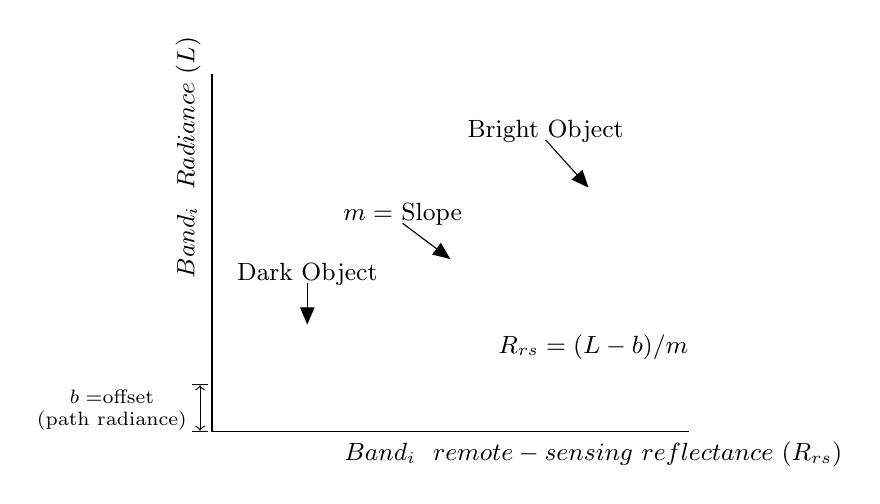
\begin{tikzpicture}[x=4ex,y=1ex]
 	%axis
	\draw (0,0) -- coordinate (x axis mid) (10,0);
    \draw (0,0) -- coordinate (y axis mid) (0,30);
 
    %labels      
	\node[below=0ex] at (8,0) {\small $Band_i~~remote-sensing~reflectance~(R_{rs})$};
	\node[rotate=90] at (-.5,23) {\small $Band_i~~Radiance~(L)$};

	\node[below=.2ex] at (-2.1,4.5) {\scriptsize $b=$offset};
	\node[below=1.4ex] at (-2.1,4.0) {\scriptsize (path radiance)};
	\draw[rotate=90,|<->|] (0,1) -- coordinate (x axis mid) (1,1);

	\node[below=0ex] at (2,15) {\small Dark Object};
	\draw[arrows=-triangle 45] (2,12.5) -- (2,9);

	\node[below=0ex] at (4,20) {\small $m=$ Slope};
	\draw[arrows=-triangle 45] (4,17.5) -- (5,14.5);

	\node[below=0ex] at (7,27) {\small Bright Object};
	\draw[arrows=-triangle 45] (7,24.5) -- (7.9,20.5);

	\node[below=0ex] at (8,9) {\small $R_{rs}=(L-b)/m$};

	%plots
	\draw plot 
		file {linereg.data};
	\draw plot[mark=*] 
		file {linereg2.data};

\end{tikzpicture}
\caption{MoB-ELM atmospheric correction method. The MoB-ELM method is based on the traditional empirical line method (ELM). Two pixels from the image, the bright and dark pixel, are used to solve a liner regression with a slope $m$ and offset $b$ in the $R_{rs}$, $L$ space. Once this relationship is established, each $L$ value in the image can be converted to $R_{rs}$ through $R_{rs}=(L-b)/m$. \label{fig:ELMregression}}
\end{figure}

\begin{figure}[htb]
  \begin{minipage}[c]{0.48\linewidth}
    \centering
      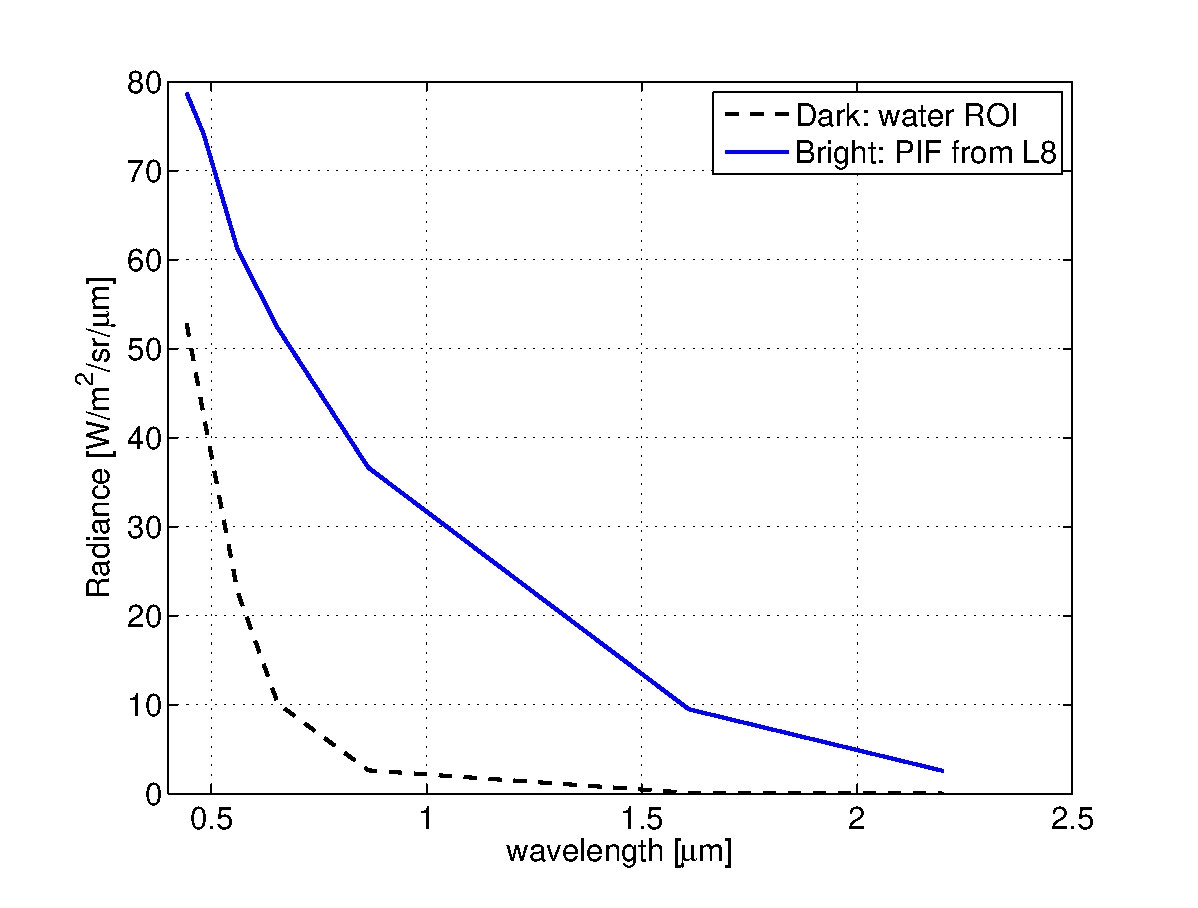
\includegraphics[width=8cm]{./Images/ELMrad130929_150422}
    % \vspace{1.5cm}
    \centerline{(a)}\medskip
  \end{minipage}
  \hfill
  \begin{minipage}[d]{0.48\linewidth}
    \centering
      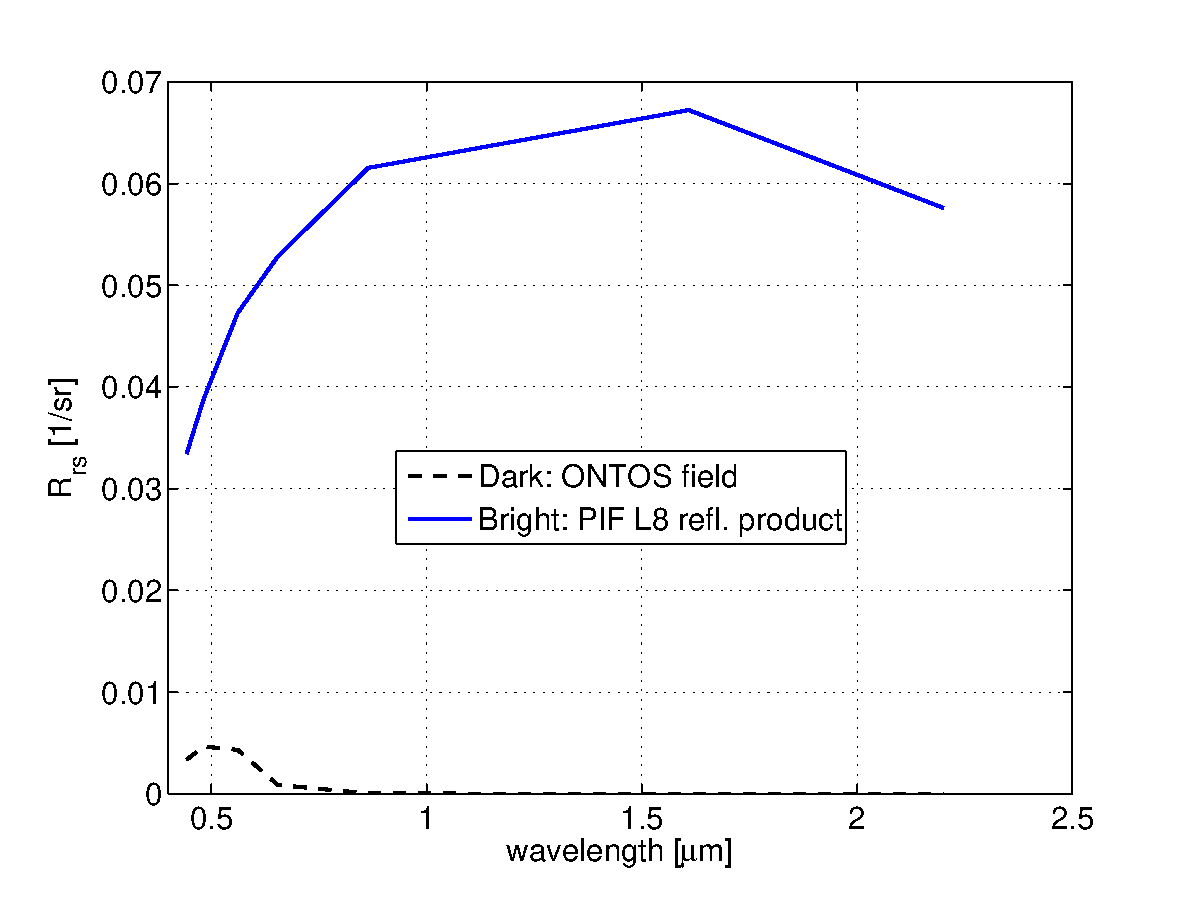
\includegraphics[width=8cm]{./Images/ELMRrs130929_150422}
    % \vspace{1.5cm}
    \centerline{(b)}\medskip
  \end{minipage}
  \caption{Example of the bright and dark pixel used in the MoB-ELM atmospheric correction method for Landsat 8 scene acquired on 09-19-2013.\label{fig:MOBELMpxls} } 
\end{figure}
% -----------------------------------------------------------
\subsection{SeaDAS-SWIR}
\label{subsec:seadasswir}
The second method analyzed in this work was the Gordon and Wang\cite{Gordon:1994} approach for atmospherically correcting satellite data over water, hereafter SeaDAS-SWIR. This method is implemented in the l2gen tool of the the Sea-viewing Wide Field-of-View Sensor (SeaWiFS) Data Analysis System (SeaDAS) software package, distributed by NASA's Ocean Biology Processing Group (OBPG) (more info: \url{http://seadas.gsfc.nasa.gov/}). The l2gen tool processes heritage Ocean-Color sensor (e.g. MODIS, SeaWiFS, OCTS or CZCS) data (Level 1) and generates Level 2 geophysical products by applying atmospheric corrections and bio-optical algorithms to the sensor. The l2gen tool includes a set of different atmospheric correction methods and variations, the Gordon and Wang's algorithm being one of them. The capability for processing OLI data was recently made fully operational in the SeaDAS version 7.2\cite{Franz:2015}. 

The atmospheric correction methods based on the Gordon and Wang's approach use standard radiative transfer methods to compute and remove scattering by the air molecules, and two bands where the water contribution is negligible to estimate the aerosol contribution for the rest of the bands. Formerly, two NIR bands were used for estimating the aerosol contribution, but a combination of NIR and SWIR bands could be used when there is some water contribution in the NIR wavelengths\cite{Wang2009}. For this analysis, The bands used for the atmospheric correction were the SWIR 1 and SWIR 2 (SeaDAS-SWIR, band 6 and 7). The OLI's NIR band was not used because the water contribution in the NIR band cannot be considered negligible due to the presence of highly turbid waters in the scene (i.e. ponds). Water has much stronger absorption at the SWIR wavelengths than at the NIR wavelengths. 

A full description of the OLI's processing in SeaDAS is described in in Ref.~\citenum{Franz:2015}. The processing in SeaDAS includes a vicarious calibration derived from the marine optical buoy (MOBY) near Lanai, Hawaii. For the atmospheric correction in SeaDAS, the option used in this study was the operational atmospheric correction scheme (aer\_opt=-2), with the shortest and longest sensor wavelength for aerosol models selection equal to band 6 and band 7 (aer\_wave\_short=1609 and aer\_wave\_long=2201). Since a default land/water mask fine enough to resolve the ponds in the scene is not included in SeaDAS, all the pixels were forced to be processed as ocean (proc\_ocean=2) and the land mask was set to the ``landmask\_null.dat'' file. Additionally, in order to increase the SNR of SWIR bands and avoid $R_{rs}$ retrieval failing in the ponds, the SWIR bands were spatially averaged with a 5x5 window. This was accomplished by including a filter (filter\_opt=1) and modifying the default SeaDAS's file ``msl12\_filter.dat''.
% -----------------------------------------------------------
\subsection{Acolite-SWIR}
The third atmospheric correction method analyzed was the implementation of the Gordon and Wang\cite{Gordon:1994}'s approach in the atmospheric correction for OLI lite (Acolite) tool (more info: \url{http://odnature.naturalsciences.be/remsem/software-and-data/acolite}). Acolite is a binary distribution of the OLI processing developed by the Royal Belgian Institute of Natural Science (RBINS). Acolite was used as a clone for the SeaDAS-SWIR method described above in \S~\ref{subsec:seadasswir}. Therefore, the option used was the default ``SWIR atmospheric correction'' with the ``Franz Ave'' gains for the vicarious calibration\cite{Franz:2015}.
% -----------------------------------------------------------
\subsection{SeaDAS-MUMM}
The fourth method evaluated in this work was the Ruddick {\it et al.}'s atmospheric correction approach\cite{Ruddick:2000bs}, hereafter SeaDAS-MUMM (MUMM: Management Unit of the North Sea Mathematical Models). This method is a modification of Gordon and Wang's algorithm\cite{Gordon:1994} for use over turbid coastal and inland waters (Case 2) or high productive Case 1 waters. In this study, this method was applied using its implementation available in SeaDAS (aer\_opt=-10), using bands 4 and 5 and setting the calibration parameter $\alpha=8.7$ for OLI, as suggested by Ref.~\citenum{Vanhellemont2014} and Ref.~\citenum{Vanhellemont2014a}. 
          % -10: Multi-scattering with MUMM correction
          %      and MUMM NIR calculation


%%%%%%%%%%%%%%%%%%%%%%%%%%%%%%%%%%%%%%%%%%%%%%%%%%%%%%%%%%%%%
\section{Chlorophyll-{\it a} RETRIEVAL}
\label{sec:chlretrieval}
% -----------------------------------------------------------
\subsection{Spectral Matching and LUT Approach}
\label{subsec:LUTapproach}
The first chlorophyll-{\it a} retrieval algorithm used in this study was the algorithm developed by Concha and Schott\cite{Concha2013IGARSS}. This algorithm uses a spectrum-matching and look-up-table (LUT) methodology to extract CPA concentrations from $R_{rs}$ data. A LUT of $R_{rs}$ spectra is created in Hydrolight\cite{MobleyHE} with IOPs and CPA concentrations measured in the field as inputs. The parameters used to create this LUT are shown in \autoref{tab:LUTconc}.

\begin{table}[htb]
\caption{Input parameters for the LUT generation in Hydrolight for the Landsat 8 image acquired on 09-19-2013. \label{tab:LUTconc}} 
\vspace{.07cm}
\small
\centering
    \begin{tabular}{ccccc}
    \hline \hline
            IOPs Input & \bfseries{$C_a$} & \bfseries{$TSS$} & \bfseries{$a_{CDOM}(440nm)$} & \bfseries{$b_b/b$}    \\
                   & $[mg~m^{-3}]$        & $[g~m^{-3}]$       &  $[1/m]$           & $[\%]$            \\ \hline \hline
\multirow{8}{*}{ONTNS}  &  0.1    	& 1.0     &  0.11   &  0.3  \\
   	&  0.5    	& 2.0   &  0.15   	&  0.4  \\
    &  1.0    	& 5.0   &  0.21   	&  0.5  \\
    &  3.0    	& 10.0  &  0.6    	&  0.6  \\ 
    &  10.0     & --    &  --   	&  0.7  \\  
    &  20.0     & --    &  --   	&  1.0  \\  
    &  40.0     & --    &  --   	&  1.4  \\
    &  --       & --    &  --   	&  2.0  \\ \hline

\multirow{8}{*}{LONGS}   &  60.0   & 25.0    &  1.0    &  0.3  \\
    &  90.0   & 45.0    &  1.2    &  0.4  \\
    &  110.0  & 50.0    &  --     &  0.5  \\
    &  --     & --      &  --     &  0.6  \\  
    &  --     & --      &  --     &  0.7  \\  
    &  --     & --      &  --     &  1.0  \\   
    &  --     & --      &  --     &  1.4  \\  
    &  --     & --      &  --     &  2.0  \\  \hline \hline
% --      &  135.0  & --      &  --     &  --   \\  
% --      &  150.0  & --      &  --     &  --   \\ \hline 
    \end{tabular}
  \end{table}

Then, this algorithm finds the closest match in the least-squared sense for the $R_{rs}$ of water pixels with unknown CPA concentrations in the LUT of water pixels with known CPA concentrations. At this point, the closest element has discrete CPA concentration values corresponding to values used for the LUT generation (see \autoref{tab:LUTconc}). Finally, a non-linear interpolation is used to interpolate between the closest match's neighbors in order to obtain continuous values for the three CPAs simultaneously. In this study, this algorithm was applied to the $R_{rs}$'s results from the MoB-ELM method only.
% -----------------------------------------------------------
\subsection{Bio-Optical Algorithm}
\label{subsec:bioopticalapproach}
The second chlorophyll-{\it a} retrieval algorithm was the standard NASA algorithm OC3\cite{OReilly2000}, which is a three-band empirical $R_{rs}(\lambda)$ band ratio algorithm, as suggested by Franz {\it et al.}(2015)\cite{Franz:2015}. Band ratio algorithms try to find a good fit between a band ratio $R$ and $C_a$. The chlorophyll-{\it a} results from the OC3 algorithm were obtained from the l2gen tool in SeaDAS when the SeaDAS-SWIR and SeaDAS-MUMM results were generated. Additionally, The OC3 algorithm was applied to the Acolite-SWIR results using the band math tool in SeaDAS. For the OLI case, the OC3 algorithm uses band 1 ($443nm$) or band 2 ($483nm$), and band 3 ($561nm$) for the band ratio, i.e.

\begin{equation}
\begin{gathered}
	C_a = 10^{\gamma}\\
	\gamma = a_0+a_1\chi+a_2\chi^2+a_3\chi^3+a_4\chi^4\\
	\chi = log_{10}(R)\\
	R = \frac{max(R_{rs}(443,483))}{R_{rs}(561)}
\end{gathered}
\end{equation}

\noindent where $a_0-a_4$ are the empirical regression coefficients. The empirical coefficients used in this study were the tuned values for OLI provided in SeaDAS (chloc3\_coef = [0.2412,-2.0546,1.1776,-0.5538,-0.4570]).

%%%%%%%%%%%%%%%%%%%%%%%%%%%%%%%%%%%%%%%%%%%%%%%%%%%%%%%%%%%%%
\section{RESULTS AND DISCUSSION}
\label{sec:results}  % \label{} allows reference to this section
% -----------------------------------------------------------
\subsection{Comparison of Rrs}
The four atmospheric correction methods (MoB-ELM, SeDAS-SWIR, Acolite-SWIR and SeaDAS-MUMM) described in Section~\ref{sec:atmcorr} are compared in this section. These algorithm were applied to the 09-19-2013 Landsat 8 image. A mask was created to mask out all pixels but water pixels. These mask was created by thresholding the Landsat 8's SWIR 2 band. \autoref{fig:Rrs443} and \autoref{fig:Rrs561} show the $R_{rs}$ for band 1 and 3 for these methods. When analyzed visually, the similarities among the methods are higher in band 3 than band 1. For band 1, SeaDAS-SWIR and SeaDAS-MUMM look similar in both the lake and ponds. Also, the SeaDAS-SWIR method exhibits some noise in band 1. This is caused due to the low SNR in SWIR bands used for the atmospheric correction. Note that there are some bottom effect in the lake's shoreline causing all methods to retrieve high $R_{rs}$ in those areas, which is not the case. This should be taken in account for future processing by masking the areas where the water are clear to enough that the bottom can be seen.

Another comparison of $R_{rs}$ at $443nm$ and $561nm$ among all four atmospheric correction methods is shown in \autoref{fig:13262Rrs443} and \autoref{fig:13262Rrs561} as scatter plots with regression line in red solid lines. Again, all the methods show more similarities in band 3 than band 1, which is corroborated by the smaller offset values for band 3 than band 1, which translates to more closeness to the $1:1$ line. This indicates that there are a higher correlation for band 3 than band 1 for all methods. \autoref{tab:RrsCompMethod} shows the slope and offset for the regression lines and the goodness of fit $R^2$ values for the comparison among all methods and for all bands. The $R^2$ values show a good correlation for all cases in the range from $0.7090$ to $0.9302$\todo{highlight min and max values in table}. \autoref{tab:RrsCompMethod} also shows the number of valid pixels retrieved $N$ and the root mean squared error (RMSE) between the methods compared. 

All methods produced negative $R_{r}$ values. This negative values indicates that the atmosphere contribution has been over estimated. These negative values are shown in \autoref{tab:RrsCompMethod} as percentage of the total of water pixels for each method compared. These negative values were not used in the comparison. Finally, \autoref{tab:RrsCompMethod} shows the percentage of total number of water pixels used in the comparison (labeled as Used $[\%]$). It can be seen that the Gordon and Wang's based methods generate more negative values compared with the MoB-ELM method overall. 

\autoref{fig:13262RrsCompField} shows a comparison between $R_{rs}$ spectra measured in the field (blue dashed line) with retrieved $R_{rs}$ spectra from the four atmospheric correction methods for different sites within the study area. The spectra for each method tend to differ more from the field spectra in band 1 and 2 than in band 3 and 4, for all sites. We calculated the normalized root mean squared error (NRMSE) for $R_{rs}(\lambda)$ to evaluate the differences between field measurements and spectra retrieved from the atmospheric correction methods methods. The NRMSE is defined as

\begin{equation}
\label{eq:NRMSE}
	NRMSE =\frac{\sqrt{\frac{1}{N}\sum_{n=1}^N{\left[R_{rs}(\lambda)_{ret}(n) - R_{rs}(\lambda)_{mea}(n)\right]^2}}}{max\{R_{rs}(\lambda)_{mea}(n)\} - min\{R_{rs}(\lambda)_{mea}(n)\}}\times100 ~[\%]
\end{equation}

\noindent where $R_{rs}(\lambda)_{ret}$ is the retrieved $R_{rs}(\lambda)$, $R_{rs}(\lambda)_{mea}$ is the measured $R_{rs}(\lambda)$, and $n=1\dots N$ is the number of measured concentrations. \autoref{fig:NRMSE130919_RRS} shows the NRMSE for all the atmospheric correction methods for all bands. It can be seen that the MoB-ELM perform the best for all bands, followed by SeaDAS-SWIR. The biggest errors are obtained when applying the Acolite-SWIR method, specially in band 1.

More data have been acquired and further validation is needed\todo{finish idea}.

% \begin{figure}[htbp!]
%   \centering
%   \includegraphics[height=8.0cm]{./Images/Collated2013262_2_band_1_D.png}
%   \caption{$R_{rs}$ for the sites for the 09-19-2013 collection after applying the MoB-ELM atmospheric correction (Labels: LONGS: Long Pond south, CRANB: Cranberry Pond, ONTOS: Lake Ontario off-shore, and ONTNS: Lake Ontario near-shore).\label{fig:RrsROIs130919} } 
% \end{figure}

% \begin{overpic}[width=0.5\textwidth,grid,tics=10]{pictures/baum}
%  \put (20,85) {\huge$\displaystyle\gamma$}
% \end{overpic}
%^^^^^^^^^^^^^^^^^^^  FIGURE ^^^^^^^^^^^^^^^^^^^^^^^^^^^^^^^^^^^^^^^^^^^^
\begin{figure}[htbp!]
	\begin{minipage}[c]{0.48\linewidth}
  		\centering
  		\begin{overpic}[trim=0 200 0 0,clip,width=7.5cm]{./Images/subset_0_of_Collocated13262_ACOSWIR_MOB_SEA_Rrs_443MOBdivpi}
  		\put (5,5) {MOB-ELM}
  		\end{overpic}
  	\end{minipage}
  	\hfill
	\begin{minipage}[c]{0.48\linewidth}
  		\centering
  		\begin{overpic}[trim=0 200 0 0,clip,width=7.5cm]{./Images/subset_0_of_Collocated13262_ACOSWIR_MOB_SEA_Rrs_443ACO}
  		\put (5,5) {Acolite-SWIR}
  		\end{overpic}
  	\end{minipage}

	\begin{minipage}[c]{0.48\linewidth}
  		\centering
  		\begin{overpic}[trim=0 200 0 0,clip,width=7.5cm]{./Images/subset_0_of_Collocated13262_ACOSWIR_MOB_SEA_Rrs_443SEA}
  		\put (5,5) {SeaDAS-SWIR}
  		\end{overpic}
  	\end{minipage}
  	\hfill
	\begin{minipage}[c]{0.48\linewidth}
  		\centering
  		\begin{overpic}[trim=30 170 40 150,clip,width=7.5cm]{./Images/Collocated13262_ACOSWIR_MOB_SEA5x5_MUMM45_Rrs_443_MUMM45}
  		\put (5,5) {SeaDAS-MUMM}
  		\end{overpic}
  	\end{minipage}
  	\begin{minipage}[c]{1.0\linewidth}
  		\centering
  		\vspace{0.5cm}
  		\begin{overpic}[trim=0 0 0 0,clip,height=1.2cm]{./Images/Collocated13262_ACOSWIR_MOB_SEA5x5_MUMM45_colorbar}
  		\put (28,16) {$R_{rs}(443nm) [1/sr]$}
  		\end{overpic}
  	\end{minipage}

  \caption{Remote-sensing reflectance ($R_{rs}$) at $443nm$ from the 09-19-2013 image over the Rochester Embayment (scene LC80160302013262LGN00) processed using the MoB-ELM, SeaDAS-SWIR, Acolite-SWIR and SeaDAS-MUMM.\label{fig:Rrs443} } 
\end{figure}
% %^^^^^^^^^^^^^^^^^^^  FIGURE ^^^^^^^^^^^^^^^^^^^^^^^^^^^^^^^^^^^^^^^^^^^^
% \begin{figure}[htbp!]
% 	\begin{minipage}[c]{0.48\linewidth}
%   		\centering
%   		\begin{overpic}[trim=0 150 40 150,clip,width=7.5cm]{./Images/Collocated13262_ACOSWIR_MOB_SEA5x5_MUMM45_Rrs_483_MOB}
%   		\put (5,6) {MOB-ELM}
%   		\end{overpic}
%   	\end{minipage}
%   	\hfill
% 	\begin{minipage}[c]{0.48\linewidth}
%   		\centering
%   		\begin{overpic}[trim=0 0 40 0,clip,width=7.5cm]{./Images/Collocated13262_ACOSWIR_MOB_SEA5x5_MUMM45_Rrs_483_ACO_R_R}
%   		\put (5,5) {ACOLITE-SWIR}
%   		\end{overpic}
%   	\end{minipage}

%   	\vspace{0.7cm}

% 	\begin{minipage}[c]{0.48\linewidth}
%   		\centering
%   		\begin{overpic}[trim=0 0 40 0,clip,width=7.5cm]{./Images/Collocated13262_ACOSWIR_MOB_SEA5x5_MUMM45_Rrs_482_SEA5x5_R}
%   		\put (5,5) {SEADAS-SWIR}
%   		\end{overpic}
%   	\end{minipage}
%   	\hfill
% 	\begin{minipage}[c]{0.48\linewidth}
%   		\centering
%   		\begin{overpic}[trim=0 150 40 150,clip,width=7.5cm]{./Images/Collocated13262_ACOSWIR_MOB_SEA5x5_MUMM45_Rrs_482_MUMM45}
%   		\put (5,5) {MUMM}
%   		\end{overpic}
%   	\end{minipage}
  	

%   	\begin{minipage}[c]{1.0\linewidth}
%   		\centering
%   		\vspace{0.5cm}
%   		\begin{overpic}[trim=0 0 0 0,clip,height=1.2cm]{./Images/Collocated13262_ACOSWIR_MOB_SEA5x5_MUMM45_colorbar}
%   		\put (28,16) {$R_{rs}(482nm) [1/sr]$}
%   		\end{overpic}
%   	\end{minipage}

%   \caption{$R_{rs}$ 483.\label{fig:Rrs482} } 
% \end{figure}
%^^^^^^^^^^^^^^^^^^^  FIGURE ^^^^^^^^^^^^^^^^^^^^^^^^^^^^^^^^^^^^^^^^^^^^
\begin{figure}[htbp!]
	\begin{minipage}[c]{0.48\linewidth}
  		\centering
  		\begin{overpic}[trim=0 155 40 150,clip,width=7.5cm]{./Images/Collocated13262_ACOSWIR_MOB_SEA5x5_MUMM45_Rrs_561_MOB}
  		\put (5,5) {MOB-ELM}
  		\end{overpic}
  	\end{minipage}
  	\hfill
	\begin{minipage}[c]{0.48\linewidth}
  		\centering
  		\begin{overpic}[trim=0 150 40 150,clip,width=7.5cm]{./Images/Collocated13262_ACOSWIR_MOB_SEA5x5_MUMM45_Rrs_561_ACO_R_R}
  		\put (5,5) {Acolite-SWIR}
  		\end{overpic}
  	\end{minipage}

  	\vspace{0.7cm}

	\begin{minipage}[c]{0.48\linewidth}
  		\centering
  		\begin{overpic}[trim=0 150 40 150,clip,width=7.5cm]{./Images/Collocated13262_ACOSWIR_MOB_SEA5x5_MUMM45_Rrs_561_SEA5x5_R}
  		\put (5,5) {SeaDAS-SWIR}
  		\end{overpic}
  	\end{minipage}
  	\hfill
	\begin{minipage}[c]{0.48\linewidth}
  		\centering
  		\begin{overpic}[trim=0 150 40 150,clip,width=7.5cm]{./Images/Collocated13262_ACOSWIR_MOB_SEA5x5_MUMM45_Rrs_561_MUMM45}
  		\put (5,5) {SeaDAS-MUMM}
  		\end{overpic}
  	\end{minipage}
  	

  	\begin{minipage}[c]{1.0\linewidth}
  		\centering
  		\vspace{0.5cm}
  		\begin{overpic}[trim=0 0 0 0,clip,height=1.2cm]{./Images/Collocated13262_ACOSWIR_MOB_SEA5x5_MUMM45_colorbar}
  		\put (28,16) {$R_{rs}(561nm) [1/sr]$}
  		\end{overpic}
  	\end{minipage}

  \caption{Remote-sensing reflectance ($R_{rs}$) at $561nm$ from the 09-19-2013 image over the Rochester Embayment (scene LC80160302013262LGN00) processed using the MoB-ELM, SeaDAS-SWIR, Acolite-SWIR and SeaDAS-MUMM..\label{fig:Rrs561} } 
\end{figure}
%^^^^^^^^^^^^^^^^^^^  FIGURE ^^^^^^^^^^^^^^^^^^^^^^^^^^^^^^^^^^^^^^^^^^^^
% \begin{figure}[htbp!]
% 	\begin{minipage}[c]{0.48\linewidth}
%   		\centering
%   		\begin{overpic}[trim=0 0 40 0,clip,width=7.5cm]{./Images/Collocated13262_ACOSWIR_MOB_SEA5x5_MUMM45_Rrs_655_MOB}
%   		\put (5,5) {MOB-ELM}
%   		\end{overpic}
%   	\end{minipage}
%   	\hfill
% 	\begin{minipage}[c]{0.48\linewidth}
%   		\centering
%   		\begin{overpic}[trim=0 0 40 0,clip,width=7.5cm]{./Images/Collocated13262_ACOSWIR_MOB_SEA5x5_MUMM45_Rrs_655_ACO_R_R}
%   		\put (5,5) {ACOLITE-SWIR}
%   		\end{overpic}
%   	\end{minipage}

%   	\vspace{0.7cm}

% 	\begin{minipage}[c]{0.48\linewidth}
%   		\centering
%   		\begin{overpic}[trim=0 0 40 0,clip,width=7.5cm]{./Images/Collocated13262_ACOSWIR_MOB_SEA5x5_MUMM45_Rrs_655_SEA5x5_R}
%   		\put (5,5) {SEADAS-SWIR}
%   		\end{overpic}
%   	\end{minipage}
%   	\hfill
% 	\begin{minipage}[c]{0.48\linewidth}
%   		\centering
%   		\begin{overpic}[trim=0 0 40 0,clip,width=7.5cm]{./Images/Collocated13262_ACOSWIR_MOB_SEA5x5_MUMM45_Rrs_655_MUMM45}
%   		\put (5,5) {MUMM}
%   		\end{overpic}
%   	\end{minipage}
  	

%   	\begin{minipage}[c]{1.0\linewidth}
%   		\centering
%   		\vspace{0.5cm}
%   		\begin{overpic}[trim=0 0 0 0,clip,height=1.2cm]{./Images/Collocated13262_ACOSWIR_MOB_SEA5x5_MUMM45_colorbar}
%   		\put (28,16) {$R_{rs}(655nm) [1/sr]$}
%   		\end{overpic}
%   	\end{minipage}

%   \caption{$R_{rs}$ 655.\label{fig:Rrs655} } 
% \end{figure}

% Method 1    Method 2    wl    NegTool1  NegTool2    usable  rsq_SS      rsq_corr    slope   offset      R^2         N           RMSE
% Acolite     MoB-ELM     443   0.53      0.09        97      .0.8791     0.8828      0.9444  -0.0047     0.8791      144047     0.0054
% Acolite     SeaDAS      443   0.53      76.74       98      .0.7804     0.7924      1.1437  -0.0053     0.7804      145186     0.0038
% Acolite     MUMM        443   0.53      74.41       99      .0.8554     0.8606      1.0600  -0.0032     0.8554      147730     0.0026
% SeaDAS      MoB-ELM     443   43.98     0.05        55      .0.7637     0.7776      0.8664  -0.0007     0.7637      141563     0.0019
% SeaDAS      MUMM        443   43.98     42.64       56      .0.8456     0.8516      0.9175  +0.0018     0.8456      145315     0.0014
% MUMM        MoB-ELM     443   42.64     0.05        56      .0.7474     0.7634      0.8811  -0.0018     0.7474      144947     0.0029
% Acolite     MoB-ELM     483   0.51      0.00        97      .0.9302     0.9314      0.9353  -0.0030     0.9302      144077     0.0037
% Acolite     SeaDAS      483   0.51      76.36       98      .0.8739     0.8779      1.1269  -0.0041     0.8739      145692     0.0028
% Acolite     MUMM        483   0.51      74.29       99      .0.9175     0.9192      1.0693  -0.0024     0.9175      147837     0.0018
% SeaDAS      MoB-ELM     483   43.76     0.00        55      .0.8454     0.8514      0.8547  +0.0002     0.8454      142116     0.0014
% SeaDAS      MUMM        483   43.76     42.57       56      .0.9122     0.9141      0.9441  +0.0015     0.9122      145888     0.0012
% MUMM        MoB-ELM     483   42.57     0.00        56      .0.8408     0.8471      0.8639  -0.0007     0.8408      145138     0.0022
% Acolite     MoB-ELM     561   0.44      0.00        97      .0.9044     0.9067      1.0183  -0.0011     0.9044      144192     0.0011
% Acolite     SeaDAS      561   0.44      75.56       99      .0.8233     0.8311      1.0307  -0.0013     0.8233      146761     0.0013
% Acolite     MUMM        561   0.44      74.15       100     .0.8968     0.8995      0.9663  -0.0001     0.8968      148040     0.0007
% SeaDAS      MoB-ELM     561   43.30     0.00        55      .0.7828     0.7946      1.0043  +0.0001     0.7828      143288     0.0009
% SeaDAS      MUMM        561   43.30     42.49       57      .0.8728     0.8768      0.9374  +0.0011     0.8728      147116     0.0010
% MUMM        MoB-ELM     561   42.49     0.00        56      .0.8468     0.8527      1.0611  -0.0010     0.8468      145339     0.0009
% Acolite     MoB-ELM     655   0.49      0.00        97      .0.8592     0.8641      1.1703  -0.0017     0.8592      144108     0.0013
% Acolite     SeaDAS      655   0.49      76.22       98      .0.7090     0.7301      0.9628  -0.0011     0.7090      145798     0.0014
% Acolite     MUMM        655   0.49      74.15       99      .0.7880     0.7992      0.9700  -0.0008     0.7880      147956     0.0010
% SeaDAS      MoB-ELM     655   43.68     0.00        55      .0.7708     0.7840      1.2158  -0.0004     0.7708      142375     0.0007
% SeaDAS      MUMM        655   43.68     42.49       56      .0.7964     0.8067      1.0063  +0.0004     0.7964      146144     0.0007
% MUMM        MoB-ELM     655   42.49     0.00        56      .0.6841     0.7091      1.2403  -0.0008     0.6841      145340     0.0009   
 
\begin{table}[!ht]
\vspace{.3cm}
\caption{ Comparison of the different atmospheric correction methods for retrieving $R_{rs}$ with the slope and offset for the regression lines and their respective goodness of fit values. \label{tab:RrsCompMethod} } 
\centering
\vspace{.2cm}
\scriptsize
\begin{tabular}{cllcccccccc} 
 % \bfseries{Band n} & \bfseries{$m$}      & \bfseries{$y_0$}    & \bfseries{$R^2$}     & \bfseries{$RMSE$} & $y(x=45^\circ)$   \\ \hline \hline
Band		&   Method 1      &  Method 2	  &	Slope  	&	Offset  &	$R^2 $  &	N      	&	RMSE    &\multicolumn{2}{c}{$R_{rs}<0~[\%]$}   &   Used 	 \\ 
$[nm]$		&	  		      &  		 	  &	  		&			&	   		&	     	&$[mg/m^3]$ & Method 1   	& Method 2  		   & $[\%]$		 \\	\hline \hline
\multirow{6}{*}{443}&Acolite-SWIR&MoB-ELM     &	0.9444 	&	-0.0047 &	0.8791 	&	144047  &	0.0054  &  ~0.53     	& ~0.09      		   &   97   	 \\
			&   SeaDAS-SWIR   &  MoB-ELM      &	0.8664 	&	-0.0007 &	0.7637 	&	141563  &	0.0019  &  43.98    	& ~0.05      		   &   55   	 \\
			&   SeaDAS-MUMM   &  MoB-ELM      &	0.8811 	&	-0.0018 &	0.7474 	&	144947  &	0.0029  &  42.64    	& ~0.05      		   &   56   	 \\
			&   Acolite-SWIR  &  SeaDAS-SWIR  &	1.1437 	&	-0.0053 &	0.7804 	&	145186  &	0.0038  &  ~0.53     	& 76.74     		   &   98   	 \\
			&   Acolite-SWIR  &  SeaDAS-MUMM  &	1.0600 	&	-0.0032 &	0.8554 	&	147730  &	0.0026  &  ~0.53     	& 74.41     		   &   99   	 \\
			&   SeaDAS-SWIR   &  SeaDAS-MUMM  &	0.9175 	&	~0.0018 &	0.8456 	&	145315  &	0.0014  &  43.98    	& 42.64     		   &   56   	 \\  \hline
\multirow{6}{*}{448}&Acolite-SWIR&MoB-ELM     &	0.9353 	&	-0.0030 &	0.9302 	&	144077  &	0.0037  &  ~0.51     	& ~0.00      		   &   97   	 \\
			&   SeaDAS-SWIR   &  MoB-ELM      &	0.8547 	&	~0.0002 &	0.8454 	&	142116  &	0.0014  &  43.76    	& ~0.00      		   &   55   	 \\
			&   SeaDAS-MUMM   &  MoB-ELM      &	0.8639 	&	-0.0007 &	0.8408 	&	145138  &	0.0022  &  42.57    	& ~0.00      		   &   56   	 \\ 
			&   Acolite-SWIR  &  SeaDAS-SWIR  &	1.1269 	&	-0.0041 &	0.8739 	&	145692  &	0.0028  &  ~0.51     	& 76.36     		   &   98   	 \\
			&   Acolite-SWIR  &  SeaDAS-MUMM  &	1.0693 	&	-0.0024 &	0.9175 	&	147837  &	0.0018  &  ~0.51     	& 74.29     		   &   99   	 \\
			&   SeaDAS-SWIR   &  SeaDAS-MUMM  &	0.9441 	&	~0.0015 &	0.9122 	&	145888  &	0.0012  &  43.76    	& 42.57     		   &   56   	 \\ \hline
\multirow{6}{*}{561}&Acolite-SWIR&  MoB-ELM   &	1.0183 	&	-0.0011 &	0.9044 	&	144192  &	0.0011  &  ~0.44     	& ~0.00      		   &   97   	 \\
	 		&   SeaDAS-SWIR   &  MoB-ELM      &	1.0043 	&	~0.0001 &	0.7828 	&	143288  &	0.0009  &  43.30    	& ~0.00      		   &   55   	 \\
	 		&   SeaDAS-MUMM   &  MoB-ELM      &	1.0611 	&	-0.0010 &	0.8468 	&	145339  &	0.0009  &  42.49    	& ~0.00      		   &   56   	 \\
	 		&   Acolite-SWIR  &  SeaDAS-SWIR  &	1.0307 	&	-0.0013 &	0.8233 	&	146761  &	0.0013  &  ~0.44     	& 75.56     		   &   99   	 \\
	 		&   Acolite-SWIR  &  SeaDAS-MUMM  &	0.9663 	&	-0.0001 &	0.8968 	&	148040  &	0.0007  &  ~0.44     	& 74.15     		   &   100  	 \\
	  		&   SeaDAS-SWIR   &  SeaDAS-MUMM  &	0.9374 	&	~0.0011 &	0.8728 	&	147116  &	0.0010  &  43.30    	& 42.49     		   &   57   	 \\ \hline
\multirow{6}{*}{655}&Acolite-SWIR&MoB-ELM     &	1.1703 	&	-0.0017 &	0.8592 	&	144108  &	0.0013  &  ~0.49     	& ~0.00      		   &   97   	 \\
	 		&   SeaDAS-SWIR   &  MoB-ELM      &	1.2158 	&	-0.0004 &	0.7708 	&	142375  &	0.0007  &  43.68    	& ~0.00      		   &   55   	 \\
	 		&   SeaDAS-MUMM   &  MoB-ELM      &	1.2403 	&	-0.0008 &	0.6841 	&	145340  &	0.0009  &  42.49    	& ~0.00      		   &   56   	 \\ 
	 		&   Acolite-SWIR  &  SeaDAS-SWIR  &	0.9628 	&	-0.0011 &	0.7090 	&	145798  &	0.0014  &  ~0.49     	& 76.22     		   &   98   	 \\
	 		&   Acolite-SWIR  &  SeaDAS-MUMM  &	0.9700 	&	-0.0008 &	0.7880 	&	147956  &	0.0010  &  ~0.49     	& 74.15     		   &   99   	 \\
	 		&   SeaDAS-SWIR   &  SeaDAS-MUMM  &	1.0063 	&	~0.0004 &	0.7964 	&	146144  &	0.0007  &  43.68    	& 42.49     		   &   56   	 \\
 \end{tabular}
\end{table}
%^^^^^^^^^^^^^^^^^^^  FIGURE ^^^^^^^^^^^^^^^^^^^^^^^^^^^^^^^^^^^^^^^^^^^^
\begin{figure}[htbp!]
  \begin{minipage}[c]{0.48\linewidth}
  		\centering
      \begin{overpic}[trim=0 280 0 0,clip,width=7.0cm]{./Images/2013262_ACOMOBSEAMUM_443_Acolite-SWIR_SeaDAS-MUMM.png}
      % \put (65,17) {\large A) $443nm$}
      \end{overpic}  
  \end{minipage}
  \hfill
  \begin{minipage}[d]{0.48\linewidth}
  	\centering
      \begin{overpic}[trim=0 280 0 0,clip,width=7.0cm]{./Images/2013262_ACOMOBSEAMUM_443_Acolite-SWIR_MoB-ELM.png}
      % \put (65,17) {\large B) $483nm$}
      \end{overpic}
  \end{minipage}

  \begin{minipage}[c]{0.48\linewidth}
  		\centering
      \begin{overpic}[trim=0 280 0 0,clip,width=7.0cm]{./Images/2013262_ACOMOBSEAMUM_443_Acolite-SWIR_SeaDAS-SWIR.png}
      % \put (65,17) {\large C) $561nm$}
      \end{overpic}  
  \end{minipage}
  \hfill
  \begin{minipage}[d]{0.48\linewidth}
  	\centering
      \begin{overpic}[trim=0 280 0 0,clip,width=7.0cm]{./Images/2013262_ACOMOBSEAMUM_443_SeaDAS-MUMM_MoB-ELM.png}
      % \put (65,17) {\large D) $655nm$}
      \end{overpic}
  \end{minipage}

  \begin{minipage}[c]{0.48\linewidth}
  		\centering
      \begin{overpic}[trim=0 280 0 0,clip,width=7.0cm]{./Images/2013262_ACOMOBSEAMUM_443_SeaDAS-SWIR_SeaDAS-MUMM.png}
      % \put (65,17) {\large C) $561nm$}
      \end{overpic}  
  \end{minipage}
  \hfill
  \begin{minipage}[d]{0.48\linewidth}
  	\centering
      \begin{overpic}[trim=0 280 0 0,clip,width=7.0cm]{./Images/2013262_ACOMOBSEAMUM_443_SeaDAS-SWIR_MoB-ELM.png}
      % \put (65,17) {\large D) $655nm$}
      \end{overpic}
  \end{minipage}

  \begin{minipage}[d]{1.0\linewidth}
  	\centering
      \begin{overpic}[trim=70 0 0 1470,clip,width=8.0cm]{./Images/2013262_ACOMOBSEAMUM_655_Acolite-SWIR_SeaDAS-MUMM.png}
      \end{overpic}
  \end{minipage}    

% 
  \caption{Scatter plots showing the comparison of remote-sensing reflectance ($R_{rs}$) at 443 nm, derived from the 09-29-2013 image over the Rochester Embayment (scene LC80160302013262LGN00) using the different methods. Colors denote pixel densities, the dashed black line is the 1:1 line, and the Reduced Major Axis (RMA) regression line is drawn in red. \label{fig:13262Rrs443} } 
\end{figure}



%^^^^^^^^^^^^^^^^^^^  FIGURE ^^^^^^^^^^^^^^^^^^^^^^^^^^^^^^^^^^^^^^^^^^^^
\begin{figure}[htbp!]
  \begin{minipage}[c]{0.48\linewidth}
  		\centering
      \begin{overpic}[trim=0 280 0 0,clip,width=7.0cm]{./Images/2013262_ACOMOBSEAMUM_561_Acolite-SWIR_SeaDAS-MUMM.png}
      % \put (65,17) {\large A) $443nm$}
      \end{overpic}  
  \end{minipage}
  \hfill
  \begin{minipage}[d]{0.48\linewidth}
  	\centering
      \begin{overpic}[trim=0 280 0 0,clip,width=7.0cm]{./Images/2013262_ACOMOBSEAMUM_561_Acolite-SWIR_MoB-ELM.png}
      % \put (65,17) {\large B) $483nm$}
      \end{overpic}
  \end{minipage}

  \begin{minipage}[c]{0.48\linewidth}
  		\centering
      \begin{overpic}[trim=0 280 0 0,clip,width=7.0cm]{./Images/2013262_ACOMOBSEAMUM_561_Acolite-SWIR_SeaDAS-SWIR.png}
      % \put (65,17) {\large C) $561nm$}
      \end{overpic}  
  \end{minipage}
  \hfill
  \begin{minipage}[d]{0.48\linewidth}
  	\centering
      \begin{overpic}[trim=0 280 0 0,clip,width=7.0cm]{./Images/2013262_ACOMOBSEAMUM_561_SeaDAS-MUMM_MoB-ELM.png}
      % \put (65,17) {\large D) $655nm$}
      \end{overpic}
  \end{minipage}

  \begin{minipage}[c]{0.48\linewidth}
  		\centering
      \begin{overpic}[trim=0 280 0 0,clip,width=7.0cm]{./Images/2013262_ACOMOBSEAMUM_561_SeaDAS-SWIR_SeaDAS-MUMM.png}
      % \put (65,17) {\large C) $561nm$}
      \end{overpic}  
  \end{minipage}
  \hfill
  \begin{minipage}[d]{0.48\linewidth}
  	\centering
      \begin{overpic}[trim=0 280 0 0,clip,width=7.0cm]{./Images/2013262_ACOMOBSEAMUM_561_SeaDAS-SWIR_MoB-ELM.png}
      % \put (65,17) {\large D) $655nm$}
      \end{overpic}
  \end{minipage}

  \begin{minipage}[d]{1.0\linewidth}
  	\centering
      \begin{overpic}[trim=70 0 0 1470,clip,width=8.0cm]{./Images/2013262_ACOMOBSEAMUM_655_Acolite-SWIR_SeaDAS-MUMM.png}
      \end{overpic}
  \end{minipage}    

% 
  \caption{Scatter plots showing the comparison of remote-sensing reflectance ($R_{rs}$) at 561 nm, derived from the 09-29-2013 image over the Rochester Embayment (scene LC80160302013262LGN00) using the the different methods. Colors denote pixel densities, the dashed black line is the 1:1 line, and the Reduced Major Axis (RMA) regression line is drawn in red. \label{fig:13262Rrs561} } 
\end{figure}

% %^^^^^^^^^^^^^^^^^^^  FIGURE ^^^^^^^^^^^^^^^^^^^^^^^^^^^^^^^^^^^^^^^^^^^^
% \begin{figure}[htbp!]
%   \begin{minipage}[c]{0.48\linewidth}
%   		\centering
%       \begin{overpic}[trim=250 310 250 0,clip,width=9cm]{./Images/2013262_ACOMOBSEAMUM_443_Acolite-SWIR_SeaDAS-MUMM.png}
%       \put (65,17) {\large A) $443nm$}
%       \end{overpic}  
%   \end{minipage}
%   \hfill
%   \begin{minipage}[d]{0.48\linewidth}
%   	\centering
%       \begin{overpic}[trim=250 310 250 0,clip,width=9cm]{./Images/2013262_ACOMOBSEAMUM_483_Acolite-SWIR_SeaDAS-MUMM.png}
%       \put (65,17) {\large B) $483nm$}
%       \end{overpic}
%   \end{minipage}

%   \begin{minipage}[c]{0.48\linewidth}
%   		\centering
%       \begin{overpic}[trim=250 310 250 0,clip,width=9cm]{./Images/2013262_ACOMOBSEAMUM_561_Acolite-SWIR_SeaDAS-MUMM.png}
%       \put (65,17) {\large C) $561nm$}
%       \end{overpic}  
%   \end{minipage}
%   \hfill
%   \begin{minipage}[d]{0.48\linewidth}
%   	\centering
%       \begin{overpic}[trim=250 310 250 0,clip,width=9cm]{./Images/2013262_ACOMOBSEAMUM_655_Acolite-SWIR_SeaDAS-MUMM.png}
%       \put (65,17) {\large D) $655nm$}
%       \end{overpic}
%   \end{minipage}

%   \begin{minipage}[d]{1.0\linewidth}
%   	\centering
%       \begin{overpic}[trim=70 50 0 1450,clip,width=9cm]{./Images/2013262_ACOMOBSEAMUM_655_Acolite-SWIR_SeaDAS-MUMM.png}
%       \end{overpic}
%   \end{minipage}    

% % 
%   \caption{Scatter plots showing the comparison of remote-sensing reflectance ($R_{rs}$) at 443, 483, 561, 655 and 865 nm, derived from the 09-29-2013 image over the Rochester Embayment (scene LC80160302013262LGN00) using the ACOLITE tool (x) and the MUMM algorithm (y). Colors denote pixel densities, the dashed black line is the 1:1 line, and the Reduced Major Axis (RMA) regression line is drawn in red. \label{fig:13262RrsAcolite-SWIR_SeaDAS-MUMM} } 
% \end{figure}
% %^^^^^^^^^^^^^^^^^^^  FIGURE ^^^^^^^^^^^^^^^^^^^^^^^^^^^^^^^^^^^^^^^^^^^^
% \begin{figure}[htbp!]
%   \begin{minipage}[c]{0.48\linewidth}
%   		\centering
%       \begin{overpic}[trim=250 310 250 0,clip,width=9cm]{./Images/2013262_ACOMOBSEAMUM_443_Acolite-SWIR_MoB-ELM.png}
%       \put (65,17) {\large A) $443nm$}
%       \end{overpic}  
%   \end{minipage}
%   \hfill
%   \begin{minipage}[d]{0.48\linewidth}
%   	\centering
%       \begin{overpic}[trim=250 310 250 0,clip,width=9cm]{./Images/2013262_ACOMOBSEAMUM_483_Acolite-SWIR_MoB-ELM.png}
%       \put (65,17) {\large B) $483nm$}
%       \end{overpic}
%   \end{minipage}

%   \begin{minipage}[c]{0.48\linewidth}
%   		\centering
%       \begin{overpic}[trim=250 310 250 0,clip,width=9cm]{./Images/2013262_ACOMOBSEAMUM_561_Acolite-SWIR_MoB-ELM.png}
%       \put (65,17) {\large C) $561nm$}
%       \end{overpic}  
%   \end{minipage}
%   \hfill
%   \begin{minipage}[d]{0.48\linewidth}
%   	\centering
%       \begin{overpic}[trim=250 310 250 0,clip,width=9cm]{./Images/2013262_ACOMOBSEAMUM_655_Acolite-SWIR_MoB-ELM.png}
%       \put (65,17) {\large D) $655nm$}
%       \end{overpic}
%   \end{minipage}

%   \begin{minipage}[d]{1.0\linewidth}
%   	\centering
%       \begin{overpic}[trim=70 50 0 1450,clip,width=9cm]{./Images/2013262_ACOMOBSEAMUM_655_Acolite-SWIR_MoB-ELM.png}
%       \end{overpic}
%   \end{minipage}    

% % 
%   \caption{Scatter plots showing the comparison of remote-sensing reflectance ($R_{rs}$) at 443, 483, 561, 655 and 865 nm, derived from the 09-29-2013 image over the Rochester Embayment (scene LC80160302013262LGN00) using the ACOLITE tool (x) and the MoB-ELM algorithm (y). Colors denote pixel densities, the dashed black line is the 1:1 line, and the Reduced Major Axis (RMA) regression line is drawn in red. \label{fig:13262RrsAcolite-SWIR_MoB-ELM} } 
% \end{figure}
% %^^^^^^^^^^^^^^^^^^^  FIGURE ^^^^^^^^^^^^^^^^^^^^^^^^^^^^^^^^^^^^^^^^^^^^
% \begin{figure}[htbp!]
%   \begin{minipage}[c]{0.48\linewidth}
%   		\centering
%       \begin{overpic}[trim=250 310 250 0,clip,width=9cm]{./Images/2013262_ACOMOBSEAMUM_443_Acolite-SWIR_SeaDAS-SWIR.png}
%       \put (65,17) {\large A) $443nm$}
%       \end{overpic}  
%   \end{minipage}
%   \hfill
%   \begin{minipage}[d]{0.48\linewidth}
%   	\centering
%       \begin{overpic}[trim=250 310 250 0,clip,width=9cm]{./Images/2013262_ACOMOBSEAMUM_483_Acolite-SWIR_SeaDAS-SWIR.png}
%       \put (65,17) {\large B) $483nm$}
%       \end{overpic}
%   \end{minipage}

%   \begin{minipage}[c]{0.48\linewidth}
%   		\centering
%       \begin{overpic}[trim=250 310 250 0,clip,width=9cm]{./Images/2013262_ACOMOBSEAMUM_561_Acolite-SWIR_SeaDAS-SWIR.png}
%       \put (65,17) {\large C) $561nm$}
%       \end{overpic}  
%   \end{minipage}
%   \hfill
%   \begin{minipage}[d]{0.48\linewidth}
%   	\centering
%       \begin{overpic}[trim=250 310 250 0,clip,width=9cm]{./Images/2013262_ACOMOBSEAMUM_655_Acolite-SWIR_SeaDAS-SWIR.png}
%       \put (65,17) {\large D) $655nm$}
%       \end{overpic}
%   \end{minipage}

%   \begin{minipage}[d]{1.0\linewidth}
%   	\centering
%       \begin{overpic}[trim=70 50 0 1450,clip,width=9cm]{./Images/2013262_ACOMOBSEAMUM_655_Acolite-SWIR_SeaDAS-SWIR.png}
%       \end{overpic}
%   \end{minipage}    

% % 
%   \caption{Scatter plots showing the comparison of remote-sensing reflectance ($R_{rs}$) at 443, 483, 561, 655 and 865 nm, derived from the 09-29-2013 image over the Rochester Embayment (scene LC80160302013262LGN00) using the ACOLITE tool (x) and the SeaDAS algorithm (y). Colors denote pixel densities, the dashed black line is the 1:1 line, and the Reduced Major Axis (RMA) regression line is drawn in red. \label{fig:13262RrsAcolite-SWIR_SeaDAS} } 
% \end{figure}
% %^^^^^^^^^^^^^^^^^^^  FIGURE ^^^^^^^^^^^^^^^^^^^^^^^^^^^^^^^^^^^^^^^^^^^^
% \begin{figure}[htbp!]
%   \begin{minipage}[c]{0.48\linewidth}
%   		\centering
%       \begin{overpic}[trim=250 310 250 0,clip,width=9cm]{./Images/2013262_ACOMOBSEAMUM_443_SeaDAS-MUMM_MoB-ELM.png}
%       \put (65,17) {\large A) $443nm$}
%       \end{overpic}  
%   \end{minipage}
%   \hfill
%   \begin{minipage}[d]{0.48\linewidth}
%   	\centering
%       \begin{overpic}[trim=250 310 250 0,clip,width=9cm]{./Images/2013262_ACOMOBSEAMUM_483_SeaDAS-MUMM_MoB-ELM.png}
%       \put (65,17) {\large B) $483nm$}
%       \end{overpic}
%   \end{minipage}

%   \begin{minipage}[c]{0.48\linewidth}
%   		\centering
%       \begin{overpic}[trim=250 310 250 0,clip,width=9cm]{./Images/2013262_ACOMOBSEAMUM_561_SeaDAS-MUMM_MoB-ELM.png}
%       \put (65,17) {\large C) $561nm$}
%       \end{overpic}  
%   \end{minipage}
%   \hfill
%   \begin{minipage}[d]{0.48\linewidth}
%   	\centering
%       \begin{overpic}[trim=250 310 250 0,clip,width=9cm]{./Images/2013262_ACOMOBSEAMUM_655_SeaDAS-MUMM_MoB-ELM.png}
%       \put (65,17) {\large D) $655nm$}
%       \end{overpic}
%   \end{minipage}

%   \begin{minipage}[d]{1.0\linewidth}
%   	\centering
%       \begin{overpic}[trim=70 50 0 1450,clip,width=9cm]{./Images/2013262_ACOMOBSEAMUM_655_SeaDAS-MUMM_MoB-ELM.png}
%       \end{overpic}
%   \end{minipage}    

% % 
%   \caption{Scatter plots showing the comparison of remote-sensing reflectance ($R_{rs}$) at 443, 483, 561, 655 and 865 nm, derived from the 09-29-2013 image over the Rochester Embayment (scene LC80160302013262LGN00) using the MUMM algorithm in SeaDAS (x) and the MoB-ELM algorithm (y). Colors denote pixel densities, the dashed black line is the 1:1 line, and the Reduced Major Axis (RMA) regression line is drawn in red. \label{fig:13262RrsSeaDAS-MUMM_MoB-ELM} } 
% \end{figure}
% %^^^^^^^^^^^^^^^^^^^  FIGURE ^^^^^^^^^^^^^^^^^^^^^^^^^^^^^^^^^^^^^^^^^^^^
% \begin{figure}[htbp!]
%   \begin{minipage}[c]{0.48\linewidth}
%   		\centering
%       \begin{overpic}[trim=250 310 250 0,clip,width=9cm]{./Images/2013262_ACOMOBSEAMUM_443_SeaDAS-SWIR_SeaDAS-MUMM.png}
%       \put (65,17) {\large A) $443nm$}
%       \end{overpic}  
%   \end{minipage}
%   \hfill
%   \begin{minipage}[d]{0.48\linewidth}
%   	\centering
%       \begin{overpic}[trim=250 310 250 0,clip,width=9cm]{./Images/2013262_ACOMOBSEAMUM_483_SeaDAS-SWIR_SeaDAS-MUMM.png}
%       \put (65,17) {\large B) $483nm$}
%       \end{overpic}
%   \end{minipage}

%   \begin{minipage}[c]{0.48\linewidth}
%   		\centering
%       \begin{overpic}[trim=250 310 250 0,clip,width=9cm]{./Images/2013262_ACOMOBSEAMUM_561_SeaDAS-SWIR_SeaDAS-MUMM.png}
%       \put (65,17) {\large C) $561nm$}
%       \end{overpic}  
%   \end{minipage}
%   \hfill
%   \begin{minipage}[d]{0.48\linewidth}
%   	\centering
%       \begin{overpic}[trim=250 310 250 0,clip,width=9cm]{./Images/2013262_ACOMOBSEAMUM_655_SeaDAS-SWIR_SeaDAS-MUMM.png}
%       \put (65,17) {\large D) $655nm$}
%       \end{overpic}
%   \end{minipage}

%   \begin{minipage}[d]{1.0\linewidth}
%   	\centering
%       \begin{overpic}[trim=70 50 0 1450,clip,width=9cm]{./Images/2013262_ACOMOBSEAMUM_655_SeaDAS-SWIR_SeaDAS-MUMM.png}
%       \end{overpic}
%   \end{minipage}    

% % 
%   \caption{Scatter plots showing the comparison of remote-sensing reflectance ($R_{rs}$) at 443, 483, 561, 655 and 865 nm, derived from the 09-29-2013 image over the Rochester Embayment (scene LC80160302013262LGN00) using the SeaDAS tool (x) and the MUMM algorithm  in SeaDAS (y). Colors denote pixel densities, the dashed black line is the 1:1 line, and the Reduced Major Axis (RMA) regression line is drawn in red. \label{fig:13262RrsSeaDAS_SeaDAS-MUMM} } 
% \end{figure}
% %^^^^^^^^^^^^^^^^^^^  FIGURE ^^^^^^^^^^^^^^^^^^^^^^^^^^^^^^^^^^^^^^^^^^^^
% \begin{figure}[htbp!]
%   \begin{minipage}[c]{0.48\linewidth}
%   		\centering
%       \begin{overpic}[trim=250 310 250 0,clip,width=9cm]{./Images/2013262_ACOMOBSEAMUM_443_SeaDAS-SWIR_MoB-ELM.png}
%       \put (65,17) {\large A) $443nm$}
%       \end{overpic}  
%   \end{minipage}
%   \hfill
%   \begin{minipage}[d]{0.48\linewidth}
%   	\centering
%       \begin{overpic}[trim=250 310 250 0,clip,width=9cm]{./Images/2013262_ACOMOBSEAMUM_483_SeaDAS-SWIR_MoB-ELM.png}
%       \put (65,17) {\large B) $483nm$}
%       \end{overpic}
%   \end{minipage}

%   \begin{minipage}[c]{0.48\linewidth}
%   		\centering
%       \begin{overpic}[trim=250 310 250 0,clip,width=9cm]{./Images/2013262_ACOMOBSEAMUM_561_SeaDAS-SWIR_MoB-ELM.png}
%       \put (65,17) {\large C) $561nm$}
%       \end{overpic}  
%   \end{minipage}
%   \hfill
%   \begin{minipage}[d]{0.48\linewidth}
%   	\centering
%       \begin{overpic}[trim=250 310 250 0,clip,width=9cm]{./Images/2013262_ACOMOBSEAMUM_655_SeaDAS-SWIR_MoB-ELM.png}
%       \put (65,17) {\large D) $655nm$}
%       \end{overpic}
%   \end{minipage}

%   \begin{minipage}[d]{1.0\linewidth}
%   	\centering
%       \begin{overpic}[trim=70 50 0 1450,clip,width=9cm]{./Images/2013262_ACOMOBSEAMUM_655_SeaDAS-SWIR_MoB-ELM.png}
%       \end{overpic}
%   \end{minipage}    

% % 
%   \caption{Scatter plots showing the comparison of remote-sensing reflectance ($R_{rs}$) at 443, 483, 561, 655 and 865 nm, derived from the 09-29-2013 image over the Rochester Embayment (scene LC80160302013262LGN00) using the SeaDAS tool (x) and the MoB-ELM algorithm (y). Colors denote pixel densities, the dashed black line is the 1:1 line, and the Reduced Major Axis (RMA) regression line is drawn in red. \label{fig:13262RrsSeaDAS_MoB-ELM} } 
% \end{figure}

%^^^^^^^^^^^^^^^^^^^  FIGURE ^^^^^^^^^^^^^^^^^^^^^^^^^^^^^^^^^^^^^^^^^^^^
\begin{figure}[htbp!]
  \begin{minipage}[c]{0.48\linewidth}
  		\centering
      \begin{overpic}[trim=0 0 0 0,clip,width=7cm]{./Images/RrsCompONTNS.png}
      \put (20,60) {A) ONTNS} 
      \end{overpic}  
  \end{minipage}
  \hfill
  \begin{minipage}[d]{0.48\linewidth}
  	\centering
      \begin{overpic}[trim=0 0 0 0,clip,width=7cm]{./Images/RrsCompONTOS.png}
      \put (20,14) {B) ONTOS}  	 	
      \end{overpic}
  \end{minipage}
  
  \begin{minipage}[d]{0.48\linewidth}
  	\centering
      \begin{overpic}[trim=0 0 0 0,clip,width=7cm]{./Images/RrsCompONTEX.png}
      \put (20,14) {C) ONTEX}  	
      \end{overpic}
  \end{minipage}
	\hfill
  \begin{minipage}[c]{0.48\linewidth}
  		\centering
      \begin{overpic}[trim=0 0 0 0,clip,width=7cm]{./Images/RrsCompRVRPL.png}
      \put (20,14) {D) RVRPLM}  		
      \end{overpic}  
  \end{minipage}

  \begin{minipage}[c]{1.0\linewidth}
  		\centering
      \begin{overpic}[trim=0 0 0 0,clip,width=7cm]{./Images/RrsCompRVRPI.png}
      \put (20,14) {E) RVRPIER}  		
      \end{overpic}  
  \end{minipage}
  % \hfill
  % \begin{minipage}[d]{0.48\linewidth}
  % 	\centering
  %     \begin{overpic}[trim=0 0 0 0,clip,width=7cm]{./Images/RrsCompLONGN.png}
  %     \put (20,60) {F) LONGN}  	
  %     \end{overpic}
  % \end{minipage}

  % \begin{minipage}[d]{0.48\linewidth}
  % 	\centering
  %     \begin{overpic}[trim=0 0 0 0,clip,width=7cm]{./Images/RrsCompLONGS.png}
  %     \put (20,60) {G) LONGS}
  %     \end{overpic}
  % \end{minipage}
  % \hfill
  %  \begin{minipage}[c]{0.48\linewidth}
  % 		\centering
  %     \begin{overpic}[trim=0 0 0 0,clip,width=7cm]{./Images/RrsCompCRANB.png}
  %     \put (45,14) {H) CRANB}  		
  %     \end{overpic}  
  % \end{minipage}

  % \begin{minipage}[d]{0.48\linewidth}
  % 	\centering
  %     \begin{overpic}[trim=0 0 0 0,clip,width=7cm]{./Images/RrsCompBRADI.png}
  %     \put (45,14) {I) BRADIN}
  %     \end{overpic}
  % \end{minipage}
  % \hfill
  % \begin{minipage}[d]{0.48\linewidth}
  % 	\centering
  %     \begin{overpic}[trim=0 0 0 0,clip,width=7cm]{./Images/RrsCompBRADO.png}
  %     \put (45,14) {J) BRADONT}
  %     \end{overpic}
  % \end{minipage}    

% 
  \caption{Comparison of $R_{rs}$ spectra for the sites on the 90-19-2013 collection. \label{fig:13262RrsCompField}} 
\end{figure}


%^^^^^^^^^^^^^^^^^^^  FIGURE ^^^^^^^^^^^^^^^^^^^^^^^^^^^^^^^^^^^^^^^^^^^^

\begin{figure}[htbp!]
  \begin{minipage}[c]{0.48\linewidth}
  		\centering
      \begin{overpic}[trim=110 0 140 0,clip,width=8.5cm]{./Images/NRMSE_RRS_B1.png}
      \put (20,40) {A) 443nm} 
      \end{overpic}  
  \end{minipage}
  \hfill
  \begin{minipage}[d]{0.48\linewidth}
  	\centering
      \begin{overpic}[trim=110 0 140 0,clip,width=8.5cm]{./Images/NRMSE_RRS_B2.png}
      \put (20,40) {B) 483nm}  	 	
      \end{overpic}
  \end{minipage}

    \begin{minipage}[c]{0.48\linewidth}
  		\centering
      \begin{overpic}[trim=110 0 140 0,clip,width=8.5cm]{./Images/NRMSE_RRS_B3.png}
      \put (20,40) {A) 561nm} 
      \end{overpic}  
  \end{minipage}
  \hfill
  \begin{minipage}[d]{0.48\linewidth}
  	\centering
      \begin{overpic}[trim=110 0 140 0,clip,width=8.5cm]{./Images/NRMSE_RRS_B4.png}
      \put (20,40) {B) 655nm}  	 	
      \end{overpic}
  \end{minipage}

  \caption{NRMSE for $R_{rs}$ at 443, 483, 561 and 655nm.\label{fig:NRMSE130919_RRS} } 
\end{figure}

% -----------------------------------------------------------
\subsection{Comparison of Chlorophyll-{\it a}}
The next step was to apply the algorithms described in Section~\ref{sec:chlretrieval} in order to retrieve chlorophyll-{\it a} concentration ($C_a$) from the $R_{rs}$ data. The spectral matching and LUT approach was applied to the $R_{rs}$ data retrieved from the MoB-ELM, while the OC3 algorithm was applied to data obtained from the rest of the algorithms. \autoref{fig:chlor_amaps} shows the $C_a$ maps obtained with the different methods. All the methods behave in a similar way for the clear water (lake), although some variability could be not visually noticeable due to the way the image is displayed. For the more turbid waters (ponds), the algorithms differ quite significant. \autoref{fig:13262RrsMeaVSRet} shows a scatterplot of $C_a$ measured in the field versus the retrieved $C_a$ from the different algorithms. It can be seen that the retrieved values obtained from the MoB-ELM algorithm are closer to the measured values than the rest of the algorithms for the higher concentrations. Similarly, we calculated the normalized root mean squared error (NRMSE) for $C_a$, defined as

\begin{equation}
\label{eq:NRMSEchl}
	NRMSE =\frac{\sqrt{\frac{1}{N}\sum_{n=1}^N{\left[C_{ret}(n) - C_{mea}(n)\right]^2}}}{max\{C_{mea}(n)\} - min\{C_{mea}(n)\}}\times100 ~[\%]
\end{equation}

\noindent where $C_{ret}$ is the retrieved concentration, $C_{mea}$ is the measured concentration, and $n=1\dots N$ is the number of measured concentrations. The NRMSE for the $C_a$ for each algorithm are shown in \autoref{fig:NRMSE130919CHL}. The best results are obtained from the MoB-ELM method with values less than $10\%$, when compared with the rest of the methods with values more than $30\%$.
%-------------
%^^^^^^^^^^^^^^^^^^^  FIGURE ^^^^^^^^^^^^^^^^^^^^^^^^^^^^^^^^^^^^^^^^^^^^
\begin{figure}[htbp!]
	\begin{minipage}[c]{0.48\linewidth}
  		\centering
  		\begin{overpic}[trim=0 0 40 0,clip,width=7.5cm]{./Images/Collocated13262_ACOSWIR_MOB_SEA5x5_MUMM45_chlor_MOB_D_R_R}
  		\put (5,5) {A) MOB-ELM}
  		\end{overpic}
  	\end{minipage}
  	\hfill
	\begin{minipage}[c]{0.48\linewidth}
  		\centering
  		\begin{overpic}[trim=0 0 40 0,clip,width=7.5cm]{./Images/LC80160302013262LGN00_L2_SWIR_FranzAve_chlor_a_ACO_OC3def}
  		\put (5,5) {B) Acolite-SWIR}
  		\end{overpic}
  	\end{minipage}

  	\vspace{0.7cm}

	\begin{minipage}[c]{0.48\linewidth}
  		\centering
  		\begin{overpic}[trim=0 0 40 0,clip,width=7.5cm]{./Images/Collocated13262_ACOSWIR_MOB_SEA5x5_MUMM45_chlor_a_SEA5x5_R}
  		\put (5,5) {C) SeaDAS-SWIR}
  		\end{overpic}
  	\end{minipage}
  	\hfill
	\begin{minipage}[c]{0.48\linewidth}
  		\centering
  		\begin{overpic}[trim=0 0 40 0,clip,width=7.5cm]{./Images/Collocated13262_ACOSWIR_MOB_SEA5x5_MUMM45_chlor_a_MUMM45}
  		\put (5,5) {D) SeaDAS-MUMM}
  		\end{overpic}
  	\end{minipage}
  	
  	\begin{minipage}[c]{1.0\linewidth}
  		\centering
  		\vspace{0.5cm}
  		\begin{overpic}[trim=0 0 0 0,clip,height=1.2cm]{./Images/Collocated13262_ACOSWIR_MOB_SEA5x5_MUMM45_colorbar_CHL_0_100}
  		\put (35,16) {$C_a [mg/m^3]$}
  		\end{overpic}
  	\end{minipage}

  \caption{$C_a$ retrieved from the different atmospheric correction methods: A) MoB-ELM, B) Acolite-SWIR, C) SeaDAS-SWIR and D) SeaDAS-MUMM. The spectral matching and LUT approach was applied to $R_{rs}$ data from MoB-ELM method. The OC3 method was applied to the $R_{rs}$ data from the Acolite-SWIR, SeaDAS-SWIR and SeaDAS-MUMM.\label{fig:chlor_amaps} } 
\end{figure}

%^^^^^^^^^^^^^^^^^^^  FIGURE ^^^^^^^^^^^^^^^^^^^^^^^^^^^^^^^^^^^^^^^^^^^^
\begin{figure}[htbp!]
  \begin{minipage}[c]{1.0\linewidth}
		\centering
     	\begin{overpic}[trim=0 0 0 0,clip,width=10cm]{./Images/CHLmeavsret.png}
    	\put(17,62){\includegraphics[trim=10 80 0 0,clip,width=3.5cm]{./Images/CHLmeavsretZOOM.png}}
      \end{overpic}  
  \end{minipage}
  \caption{Comparison retrieved versus measured $R_{rs}$ for the sites on the 90-19-2013 collection. \label{fig:13262RrsMeaVSRet}} 
\end{figure}
% %^^^^^^^^^^^^^^^^^^^  FIGURE ^^^^^^^^^^^^^^^^^^^^^^^^^^^^^^^^^^^^^^^^^^^^
% \begin{figure}[htbp!]
%   \begin{minipage}[c]{0.48\linewidth}
%   		\centering
%       \begin{overpic}[trim=0 250 0 0,clip,width=7cm]{./Images/2013262_ACOMOBSEAMUM_C_a_Acolite-SWIR_SeaDAS-MUMM.png}
%       \end{overpic}  
%   \end{minipage}
%   \hfill
%   \begin{minipage}[d]{0.48\linewidth}
%   	\centering
%       \begin{overpic}[trim=0 250 0 0,clip,width=7cm]{./Images/2013262_ACOMOBSEAMUM_C_a_Acolite-SWIR_MoB-ELM.png}
%       \end{overpic}
%   \end{minipage}

%   \begin{minipage}[c]{0.48\linewidth}
%   		\centering
%       \begin{overpic}[trim=0 250 0 0,clip,width=7cm]{./Images/2013262_ACOMOBSEAMUM_C_a_Acolite-SWIR_SeaDAS-SWIR.png}
%       \end{overpic}  
%   \end{minipage}
%   \hfill
%   \begin{minipage}[d]{0.48\linewidth}
%   	\centering
%       \begin{overpic}[trim=0 250 0 0,clip,width=7cm]{./Images/2013262_ACOMOBSEAMUM_C_a_SeaDAS-MUMM_MoB-ELM.png}
%       \end{overpic}
%   \end{minipage}

%   \begin{minipage}[c]{0.48\linewidth}
%   		\centering
%       \begin{overpic}[trim=0 250 0 0,clip,width=7cm]{./Images/2013262_ACOMOBSEAMUM_C_a_SeaDAS-SWIR_SeaDAS-MUMM.png}
%       \end{overpic}  
%   \end{minipage}
%   \hfill
%   \begin{minipage}[d]{0.48\linewidth}
%   	\centering
%       \begin{overpic}[trim=0 250 0 0,clip,width=7cm]{./Images/2013262_ACOMOBSEAMUM_C_a_SeaDAS-SWIR_MoB-ELM.png}
%       \end{overpic}
%   \end{minipage}

%   \begin{minipage}[d]{1.0\linewidth}
%   	\centering
%       \begin{overpic}[trim=0 0 0 1500,clip,width=7cm]{./Images/2013262_ACOMOBSEAMUM_C_a_SeaDAS-SWIR_MoB-ELM.png}
%       \end{overpic}
%   \end{minipage}    

% \vspace{.5cm}
%   \caption{$C_a$ comparison among all the four method analyzed in this work. \label{fig:13262Chlor} } 
% \end{figure}
%^^^^^^^^^^^^^^^^^^^  FIGURE ^^^^^^^^^^^^^^^^^^^^^^^^^^^^^^^^^^^^^^^^^^^^
\begin{figure}[htbp!]
  \centering
  \includegraphics[height=8.0cm]{./Images/13262_NRMSE_CHL.png}
  \caption{NRMSE for $C_a$. The $R_{rs}$ results from the MoB-ELM were used for the Concha and Schott's retrieval of $C_a$, while the results of the rest of the atmospheric correction algorithms were used for the NASA's bio-optical algorithm. The MoB-ELM results combined with the Concha and Schott's $C_a$ retrieval give the best results.\label{fig:NRMSE130919CHL} } 
\end{figure}


%%%%%%%%%%%%%%%%%%%%%%%%%%%%%%%%%%%%%%%%%%%%%%%%%%%%%%%%%%%%%
\section{Conclusions}
\label{sec:conc}  % \label{} allows reference to this section
There were four different atmospheric correction algorithms analyzed in this study. Three of them are based in the NASA's standard algorithms based on the methods developed by Gordon and Wang\cite{Gordon:1994}. The fourth algorithm is based on the MoB-ELM algorithm developed by Concha and Schott\cite{Concha2014SPIE}. The remote-sensing reflectances retrieved from these atmospheric correction algorithms were compared against each other. There are better agreements in band 3 and 4 than in bands 1 and 2 for all algorithms, which can be concluded from the RMSE (\autoref{tab:Sites}). When compared with {\it in situ} data, the MoB-ELM and Gordon and Wang's algorithm from SeaDAS (SeaDAS-SWIR) show similar results for all bands (\autoref{fig:NRMSE130919_RRS}). The results from the Gordon and Wang's algorithm from Acolite (Acolite-SWIR) shows the largest disagreement (\autoref{fig:NRMSE130919_RRS}).

When retrieved chlorophyll-{\it a} concentrations ($C_a$) are compared with {\it in situ}, the results from the Concha and Schott's approach perform so much better than the rest of the algorithms(\autoref{fig:NRMSE130919CHL}). These results show that the NASA's bio-optical algorithms fail in Case 2 waters. This was expected since these algorithms were developed with the lack of {\it in situ} data representative of Case 2 waters with high concentration of color producing agents (CPAs).

These results demonstrate that for Case 2 waters, the solution for the ocean color measurements needs to be local and not global, as opposed to Case 1 waters. This local solution, the combined MoB-ELM algorithm with Concha and Schott's $C_a$ retrieval algorithm, requires some knowledge of the waters to be studied, such as inherent optical properties (IOPs) and CPA concentration in at least one site.

Further validation needs to be done. This implies to apply the algorithms to more images and compare the results. Also, more {\it in situ} data need to be collected for comparison.
%%%%%%%%%%%%%%%%%%%%%%%%%%%%%%%%%%%%%%%%%%%%%%%%%%%%%%%%%%%%%
\acknowledgments     %>>>> equivalent to \section*{ACKNOWLEDGMENTS}       
The authors would like to extend a special thanks to the United States Geological Survey (USGS) for its sponsorship (contract number G12PC00065) that has made this effort possible.
%%%%%%%%%%%%%%%%%%%%%%%%%%%%%%%%%%%%%%%%%%%%%%%%%%%%%%%%%%%%%
%%%%% References %%%%%

\bibliography{/Users/javier/Desktop/Javier/PHD_RIT/Latex/javier_bib}   
\bibliographystyle{spiebib}   %>>>> makes bibtex use spiebib.bst


\end{document} 
